\section{Introduction}

The distribution of wealth and income has recently made a comeback to the
centre of economic discourse in advanced economies. The ongoing rise of
income inequality, observed since the early 1980s especially in Anglo-Saxon
countries, has received renewed attention in the public sphere since the
financial started taking its toll on living standards across the world. At
the same time, the best-selling book by \citet{Piketty2014} led to a surge
in interest in the role of capital in the economy, and, by extension, the
distribution of wealth, both in the academic literature and the popular
press. \\
While the broader public has only recently picked up on the issues arising
around income and wealth distributions, they have sat squarely in the centre
of many sub-fields of economics for a long time. The income distribution has
long been of interest to labour economists trying to understand the forces
shaping the evolution of earnings in the labour market, while at least the
accumulation of aggregate wealth plays a central role in macroeconomic
models of economic growth. This chapter, as well as chapter three, 
focuses on the intermediate step that takes us from an
income to a wealth distribution - economic models of household saving.
When attempting to build a model of the wealth distribution, the first
step of course is to get an understanding of the object we want to model.
To this end, this chapter starts by presenting stylised facts of the wealth
distributions in advanced countries and discusses some of the limitations
of the data available. It then builds a simple life-cycle model of consumption
and savings to guide the following discussion and fix notation. Using this
basic model, different savings motives and their importance in the context
of aggregate wealth accumulation are discussed. Following this, the role of
income uncertainty and market structure is examined in more detail.


\section{Stylised facts}
The most notable and consistent fact that emerges when looking at wealth
distributions across all countries and different time periods is that wealth
is highly unevenly distributed, much more so than income. \citet{Vermeulen2014}
argues that wealth holdings are so concentrated, that even surveys employing 
designs that feature oversampling of richer households (such as the US Survey of
Consumer Finances (SCF), or the British Wealth and Asset Survey (WAS)) 
underestimate the percentage share of wealth held by the highest percentile of the
wealth distribution by anywhere from one to five percentage points, while surveys
that don't oversample underestimate the share by up to ten percentage points.
Keeping this in mind, the een when comparing Gini indices and top shares of income and wealth, as in
Table \ref{tab:gini_topshares} or looking at histograms and cdfs of wealth and
income distributions as in Figure \ref{fig:was_wealthholdings}. It is important to note
that in producing these aggregate numbers and figures, one necessarily has
to make decisions on how exactly to construct measures of income and wealth,
which will have to be kept in mind when comparing model predictions with
empirical numbers. When constructing an income measure, the obvious starting
point are labour earnings, and for many economic applications simply
observing an individual's wages will be enough. When thinking about questions
of consumption smoothing though, we are ultimately interested in accounting
for all claims on consumption goods available to an individual or household
in a given period, and while for most people the largest part of these claims
stem from labour earnings, we will also want to account for the effect of
government programs (by constructing a post-tax, post-transfer income measure),
income from accumulated assets, and potentially even informal insurance
arrangements such as inter-vivos transfers between family and friends.
In constructing wealth measures, we again have to think closely about the
question we are trying to answer when constructing them. If the goal is to
account for all productive capital in the economy that can be used in
production, a measure of total net wealth aggregating all forms of asset and
debt classes, and including some durable consumption goods such as cars. When
thinking about the role of wealth in helping the household to smooth out
income fluctuations, it might be more appropriate to exclude very illiquid
assets such as housing, and look more closely at the role of debt for households
which might be at their borrowing constraint and are thus vulnerable to
reductions in their borrowing limit, even though their net wealth (including
illiquid assets) is positive. Finally, important questions are raised by
the existence of various government and private pension schemes, which have
to be factored in when constructing measures of a household's lifetime
resources, but whose exact value might be uncertain (for the case of defined
contribution plans) and not well understood by households themselves.


\begin{table}%
\begin{tabular}{lcr}

\end{tabular}
\caption{Measures of wealth concentration in different data sets.}
\label{tab:gini_topshares}
\end{table}

\begin{figure}
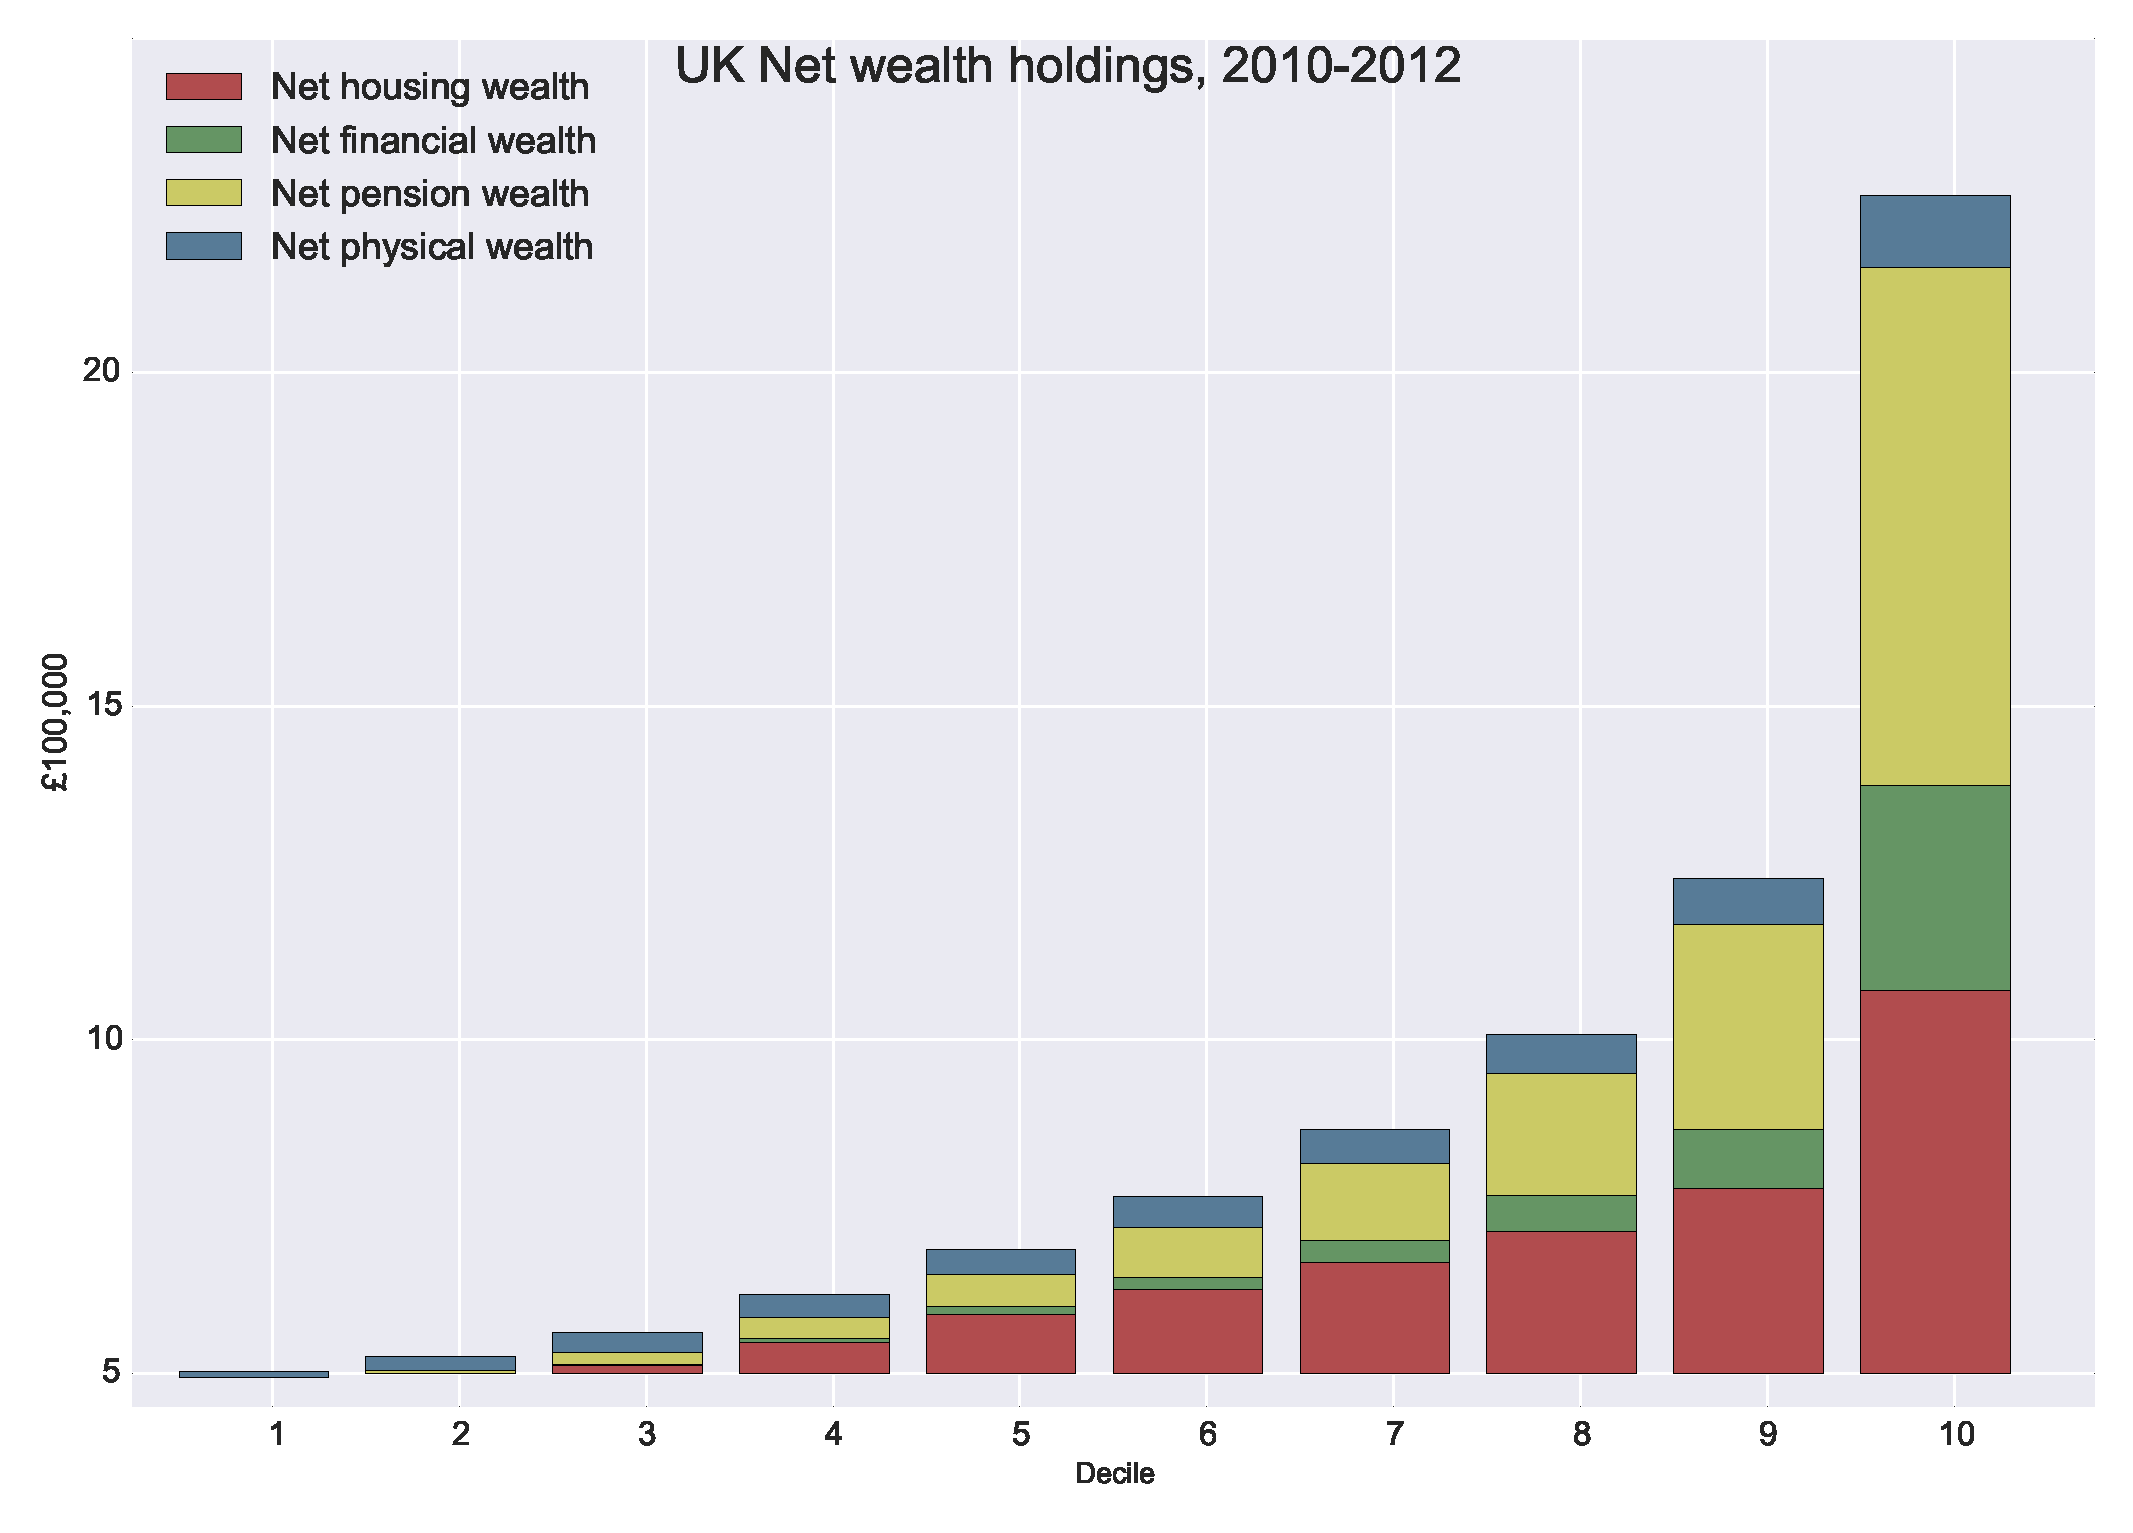
\includegraphics[width=\columnwidth]{was_wealth_holdings}
\caption{Histograms and cdfs of household net wealth in different data sets.}
\label{fig:was_wealthholdings}
\end{figure}

\section{A workhorse model}
The basic model underlying the discussion of savings behaviour and wealth 
accumulation in this chapter is the life-cycle model of household behaviour 
dating back to \citet{ModiglianiBrumberg1954} \footnote{A more detailed 
treatment of the general class of models can be found both in 
\citet{BrowningCrossley2001} and in \citet{AttanasioWeber2010}, although both 
papers have their focus on household consumption behaviour rather than wealth 
accumulation.}. The model can be written as a single household solving the 
problem

\begin{align}
\max_{\{c_{t+j}\}_{j=0}^{T-t}} \sum_{j=0}^{\infty} \delta^{t+j} \mathbb{E}_t \big[ u(c_{t+j}, z_{t+j}) \big] \label{maxprob}
\intertext{subject to} 
a_{t+1} = (1+r)(a_t + y_t - c_t) \label{bc}
\end{align}
where $T$ is the last period of the planning horizon, $\delta$ is the subjective
discount factor, $u()$ is the instantaneous felicity function -- usually assumed
to be of the CRRA form, $\frac{c^{1-\sigma}}{1-\sigma}$, where $\sigma$ is the 
coefficient of relative risk aversion --, $c$ is 
consumption, $a$ are financial assets, which allow the household to transfer 
resources across time, $r$ is a one-period interest rate, and $y$ is income. 
$z$ is used as a stand-in variable denoting the fact that households might, 
in general, care about other things that are not captured by the concept of 
current consumption; examples would be habits or durable consumption (which 
break the time-separability of the utility function), leisure time, particular 
classes of assets (such as housing) or bequests left to future generations.  
While in general, $T \rightarrow \infty$ is a possibility, and infinite horizon 
versions -- first advocated by \citet{Friedman1957} -- of the life-cycle model 
are widely used in macroeconomic applications, the finite horizon model will be 
more useful for the following discussion and forms the centrepiece of this 
thesis for a number of reasons which will become clear as we progress.

\section{Saving motives}
When trying to understand wealth distributions through the lens of the model
outlined above, the key question is: why do households save? The basic model,
in which consumers only care about the time path of instantaneous utility 
derived from consumption, suggests that households will save if and only if
it leads to preferential allocation of consumption over time -- they engage 
in consumption smoothing. As \citet{BrowningCrossley2001} point out, consumption
smoothing can happen at different frequencies, depending on the exact set-up 
of the model. In \citet{ModiglianiBrumberg1954} the main reason saving was the
existence of a retirement period, which necessitates consumption smoothing over
the life cycle -- wealth accumulation during working life to pay for consumption
in retirement. The implication of this simple model is that wealth accumulation
on the household level solely depends on the length of the retirement period, 
while in aggregate wealth accumulation crucially hinges on the growth rate
of the economy. The crucial assumption that allows Modigliani and Brumberg to
focus on consumption smoothing over the life cycle was that of constant income,
an assumption that is obviously incorrect and easily rejected by the data.


\section{Income uncertainty and market structure}
With the assumption of a non-constant income stream, it becomes important to 
think about the opportunities households have to insure themselves against
these fluctuations, or, in other words, which market structure they are facing.
To make income fluctuations relevant for the economic agent, the world of 
complete markets, in which a full set of Arrow securities covering each possible
state of the world can be bought and sold, has to be abandoned in favour of 
market \textit{incompleteness}. The most convenient, and at the same time most
extreme, departure from the complete markets assumption is to assume away any
sort of insurance markets except for very simple self-insurance through risk-
free one-period bonds. This market structure is implicit in the formulation of
the consumer problem in equation \ref{bc} -- there is just one asset for the 
household to sell or buy, and this asset has a certain payoff in the following 
period, which is not contingent on the state of the world. The big advantage of 
this setup is tractability: simple models of this kind can often be solved 
analytically, and in recursive formulations of more complex problems, the simple
market structure only adds one state variable to the problem. The drawback, 
obviously, is that this market structure is at odds with the economic reality,
where households are able to buy a hoist of different assets that vary widely 
in liquidity as well as in the degree to which payoff are state-contingent.
We defer the consideration of the role of liquidity to section \ref{housing}, 
which deals with the largest asset in most households' portfolio, housing, and
examine the role of insurance first. The basic idea when investigating the 
extent to which households have access to insurance mechanisms is to analyse
the joint dynamics of income and consumption data, and compare them with the
implications derived from models with different insurance mechanisms. In a 
complete market setup, where households can fully insure income risk, 
idiosyncratic changes in income should not translate into changes in consumption,
implying a flat profile of cross-sectional consumption inequality over the life-
cycle, irrespective of the underlying stochastic process governing income. This 
is not the case in the absence of insurance opportunities, with the opposite 
end of the model spectrum being inhabited by the Aiyagari-Bewley-Hugget-Imrohoroglu
class of models (\citet{Aiyagari1994}, \citet{Bewley1977}, \citet{Huggett1993},
\citet{Imrohoroglu1989}). These model don't feature any insurance possibilities
apart from non-contingent one-period bonds and also deliver specific predictions
on the relationship between income, consumption and savings\footnote{More precisely,
the opposite end of the insurance spectrum would be a world that does not even
offer noncontingent bonds, although this market structure is obviously not suited
to examine any interesting economic question.}. The precise predictions of the 
model for how households will consume and save depend crucially on the specification
of the stochastic process governing income uncertainty -- essentially the object
over which $\mathbb{E}$ in equation \ref{eq:maxprob} is defined. When applying an
income process consisting of permanent and transitory shocks to this model, the 
well-known\footnote{For a rigorous derivation refer to your favourite Macroeconomics
textbook, e.g. \citet{LjungqvistSargent2012}, chapter 17.} results that consumption
should react to permanent changes in income, while transitory changes in income
should be buffered by saving and dissaving in the noncontingent bond. This 
prediction of the model is exploited by some authors to elicit information on 
the decomposition of income changes into permanent and transitory shocks using 
consumption data: assuming that the model is correct, increases in income 
inequality in the data that are accompanied by contemporary increases in consumption
inequality must be induced by permanent shocks to income, while changes in the 
income distribution that do not lead to changes in the consumption distribution
can be seen to be the consequence of transitory shocks. \citet{BlundellPreston1998}
is an example of a paper employing exactly this strategy to examine data 
on consumption and income from the British Family Expenditure Survey to examine
the properties of changes in the income distribution in Britain between 1968 
and 1992. One problem of these studies however is a large literature documenting 
"excess smoothness" of consumption in the data, that is showing that consumption
does \textit{not} change one-for-one even with changes in income that are known
to be permanent (are very detailed account on the early research on this can be
found in \citealt{Deaton1992book}), implying that there are at least some 
insurance opportunities available to households in the real world. Based on the 
rejection of both full and no insurance in the data, an active literature has 
developed trying to quantify the amount of insurance households have access to.
\citet{KruegerPerri2004}
\citet{HeathcoteStoreslettenViolante2004}
\citet{HeathcoteStoreslettenViolante2007}
\citet{BlundellPistaferriPreston2008} develop a novel imputation procedure 
designed to alleviate measurement problems in PSID consumption data to test 
\citet{KaplanViolante2010} examine how to what extent the empirical estimates
of consumption insurance that \citet{BlundellPistaferriPreston2008} obtain can
be replicated in a standard incomplete market model with capital as the only 
savings vehicle. 



\section{The role of housing}\label{housing}
While much effort has been devoted to examining the implications of income risk
and market structure for wealth accumulation through precautionary savings, it 
is undeniable that a large part of household saving happens in the form of an
asset which cannot perform the role of buffering against income shocks: housing.
As figure \ref{fig:was_wealthholdings} demonstrates using data from the US SCF and
the British Wealth and Asset Survey, by far the largest share of household
portfolios is invested in housing wealth, with the notable exception of the
very richest households. The illiquidity of housing, the high transaction costs
and the consumption element of housing purchases make this asset fundamentally
different from the one-period riskless bond considered in our workhorse model.
A number of authors have considered the effects of allowing households to save
in housing assets in addition to financial assets: \citet{CampbellHercovitz2009} 
and \citet{CampbellHercovitz2005}, \citet{Yang2009}, \citet{Iacoviello2008}



\section{Closed and open economies}
One key decision when building a model of wealth accumulation is the question
of how the interest rate on savings is determined. Traditionally, the 
macroeconomic literature has viewed the interest rate as an endogenous parameter,
pinned down by the marginal product of capital from the economies production 
function and the quantity of capital available, which in turn is governed by 
household's savings decisions. In fact, the main contribution of the seminal 
work by \citet{Aiyagari1994} was to highlight the effect of idiosyncratic income
risk and borrowing constraints, two key features of the heterogeneous agent models
most frequently used to examine questions related to the wealth distribution,
on the steady state interest rate. Aiyagari shows that compared to a standard 
growth model, the steady state stock of capital in a closed incomplete markets
economy is higher, and, correspondingly, the steady state interest rate is lower
because of precautionary savings induced by income uncertainty.
Another problem introduced by endogenous interest rates is a computational one,
the determination of the interest rate requires asset market clearing, which 
implies that household savings choices have to be consistent with each other
in each period. 
For these reasons, many researchers have opted for treating the interest rate
as an exogenous parameter, set anywhere between three \citep{Cagetti2003} and
5.2 \citep{GourinchasParker2002} percent. Whether this is justified will depend
on two things: theoretically, one has to ask whether general equilibrium effects
are likely to alter the answer to the question at hand, while empirically the 
question of the elasticity of the interest rate to changes in aggregate wealth.
In general equilibrium models in the tradition of \cite{Aiyagari1994}, this 
elasticity is given by the sensitivity of the marginal product of capital to
the quantity of aggregate capital, which can be determined from the production 
function. While the Cobb-Douglas function is the function of choice in the 
literature (see e.g. \citealt{CastanedaRiosRull2003}), recent work by 
\citet{Piketty2014} casts doubt on the appropriateness of this assumption and 
argues for a functional form implying a lower elasticity of the interest rate
to increases in the capital stock. Irrespective of the choice of the production 
function though, one has to ask who valid the assumption of a closed economy, in 
which household savings have direct impacts on the quantity of productive capital
in the economy, is. Given the deep international integration of modern financial
markets, it appears that the open economy assumption often used in international
economics to describe economies that can not set interest rates might be useful
when thinking about the dynamics of interest rates in response to changes in 
saving behaviour in the local economy

\section{Wealth Distribution Papers}
In the last years, many authors have used the increasing possibilities offered
by the increase in computing power to derive an additional implication from the
broad class of incomplete market models outlined above: a simulated wealth 
distribution. While there are many practical difficulties in creating model 
outputs that can reasonably compared to the data collected in surveys (some of
which have been alluded to in the above discussion on the definition of wealth),
in principle the simulated wealth distribution derived from life-cycle models
can be used to calibrate deep parameters of the model, provide an additional
test for how well the model is able to capture household savings behaviour, 
and shed light on which mechanisms are crucial in driving the evolution of 
aggregate savings at different parts of the distribution. \\
An early attempt to use the wealth distribution to estimate the parameters of
a life-cycle model of household savings can be found in \citet{Cagetti2003},
who uses a simple model similar to the one outlined in equations \ref{maxprob}
and \ref{bc}. Important additions in his version of the model are a bequest 
motive -- which, ceteris paribus, will increase the wealth holdings of elderly
households -- and a simplified pension system, which guarantees each household
a pension depending on their education level, and thereby lowers wealth 
accumulation during working life. The idea behind the estimation strategy is 
simple: given a stochastic process for household income, the parameters $\beta$,
$\sigma$ and $\alpha$ pin down a solution to the household's savings problem 
which allows one to simulate a theoretical wealth distribution from optimal 
household behaviour. Therefore, it is possible to use the simulated method of
moments to construct an estimator that chooses the triplet $(\delta,\sigma, 
\alpha)$ which minimises the distance between empirical moments of the wealth
distribution and its simulated counterparts. Given the high skewness of wealth
data, Cagetti opts for median wealth by 5-year age group as the moment to match.
As has become clear in the previous discussion, a crucial element driving 
household choices in the model is the income risk they face, making the choice
for the stochastic process representing this risk and its calibration a crucial
step in modelling wealth distributions. Cagetti opts for a process consisting
of a trend growth component common to all households, an age-education component
estimated for CEX data, and an MA(1) process representing the stochastic nature
of income. With his calibration, Cagetti finds low degrees of persistence, with
pronounced heterogeneity across education groups, and high degrees of risk 
aversion, implying a significant contribution of precautionary savings to 
aggregate wealth. \\
A very similar exercise is performed by \citet{HintermaierKoeniger2011}, who 
construct a minimum distance estimator based on the shape of the cross-sectional
distribution of wealth at different stages of the life cycle. That is, rather
than simply targeting the 50th percentile of wealth holdings  as 
\citet{Cagetti2003}, here all percentiles of the wealth distribution from 10 
to 90 are considered. Increasing the number of moments to match leads to estimates 
of the discount factor which are an order of magnitude more precise than in 
\citet{Cagetti2003}. The estimate for the discount factor, at $\hat{\delta}=0.985$, 
is at the upper bound of the estimates in \citet{Cagetti2003}, while the 
estimated risk aversion parameter $\hat{\sigma}=1.08$ is only a third to one 
sixth as large as Cagetti's estimate, depending on the subgroup under consideration. \\
Exercises like the ones by \citet{Cagetti2003} and \citet{HintermaierKoeniger2011}
repeatedly come to one conclusion: while a simple life-cycle incomplete markets
model with idiosyncratic income shocks calibrated from income data can match 
parts of the wealth distribution well, and generate the correct ordering of 
inequality in wealth, income, and consumption -- wealth being more unequally 
distributed than income, which in turn is more unequally distributed than 
consumption -- it fails to capture the extremely high dispersion in wealth, 
especially at the top of the distribution\footnote{Indeed, this is the reason
cited in \citet{HintermaierKoeniger2011} for excluding the top decile of the 
wealth distribution from the targeted moments: the model has no chance of capturing
the extremely high net worth of the richest households, which exceeds 150 times
average yearly income in the 2007 SCF.}. 

A straightforward way of improving the fit of the more standard model is employing an
income process that features large persistent shocks with low probability, as 
first popularised by \citet{CastanedaRiosRull2003}. Their specification of the 
income process is a four-state Markov chain, the highest state of which is only
reached with very low probability, has a persistence of about five years, and
implies an income 1000 times higher than median income. In this setup, it is evident
that simple consumption smoothing considerations lead to very high savings rates
for rich households, which in turn lead to a large wealth concentration at the 
top end of the distribution. It is however questionable to what extent models 
relying on this type of income process, which cannot be reconciled with the 
evidence from micro-level surveys on household incomes, can be used to inform 
policy analysis; a recent example of this problem can be found in the work of 
\cite{KindermannKrueger2014}, who investigate optimal labour income taxation
in an Aiyagari-Bewley-Huggett style model featuring a similar income process and
validating their model by fitting the top tail of the empirical wealth distribution.
Unsurprisingly, they find very high optimal tax rates of around 90 percent on 
top earners, however this result is entirely driven by the income process used
and subsequent work by \cite{BadelHuggett2014} demonstrates that optimal tax
rates are significantly lower if one includes an earnings process based on 
human capital formation, which is parametrised to mirror the empirical evolution
of earnings dispersion.
This shows that a model that fits the wealth distribution is not necessarily 
suited for policy evaluation, especially if the good fit is the artefact of
model assumptions that have little empirical support and gives reason to 
include more realistic features of the economic environment into the model 
which might help to explain observed patterns in the data. A number of researchers
have extended the baseline model in various dimensions, some of which we will 
discuss here\footnote{The discussion here draws on the work by \cite{DeNardi2015}.}.

A more realistic version on the role of the household income process in shaping
the wealth distribution is the inclusion of entrepreneurial activity as an
alternative to labour income. \citet{Quadrini2000} is an early attempt to 
include business income in the model. His economy features infinitely lived 
households, that have the opportunity to undertake entrepreneurial activity, but
need to save up capital in order to start a business first. After having started
the business, these agents face substantially higher risk than working households,
a fact that combined with high borrowing costs and infinite lives leads to 
wealth accumulation at the top of the distribution as large as in the data. 
\citet{CagettiDeNardi2006} improve on this model by allowing for an endogenous
choice in the amount of capital invested in the business, and in their model the
potentially high rates of return on business activity are the main factor 
affecting the right tail of the wealth distribution. This aspect makes their 
model a close cousins to models that feature different rates of returns for 
different asset classes, which we turn to later. \citet{CagettiDeNardi2006}
also provide an empirical rationale for the modelling of entrepreneurial 
activity, using SCF data to show that amongst the wealthiest 1\% of households,
81\% are business owners or self employed, although this group of households 
only accounts for 17\% of all households. They also show that amongst business
owners, mean and median wealth are higher for those not actively engaged in 
managing the business, providing support for models that feature an intergenerational
transfer of assets, which we turn to next.

A successful line of research extends the model by moving from a simple life-
cycle perspective to an overlapping generations (OLG) model, in which inequalities
can be transmitted across generations and hence accumulate over time. This 
transmission mechanism can work through either assets directly, by adding 
a bequest motive to the agents utility function which prevents them from drawing
down assets in old age, or through heritability of human capital in the form 
of skills or learning ability. The role of inheritance rose to prominence in the 
empirical literature with a dispute between \citet{KotlikoffSummers1981}, who 
estimate that around 80\% of total wealth is inherited, while just 20\% is 
the result of life-cycle saving, and \citet{Modigliani1986}, who argues that the 
role of the sources of wealth accumulations is exactly reversed. Recently, Thomas
Piketty and a number of co-authors (\citealt{Piketty2011}, 
\citealt{PikettyPostelRosenthal2014}, \citealt{PikettyZucman2015}) revive this
debate using long-run time series from France and drawing on other work from 
the UK and Germany, finding large variations in the annual flow of inheritance
as a share of total wealth, but concluding that the overall importance of inheritance
in shaping the wealth distribution is closer to Kotlikoff and Summer's estimates
than to Modigliani's. The correct estimation of the role of inherited wealth is
further complicated by the possibility of inter vivos transfers, which are not
captured by inheritance tax data. This point is made forcefully by 
\citet{GaleScholz1994}, who use data on transfers from the SCF to estimate that
20 percent of aggregate wealth is passed on across generations via inter vivos
transfers (compared to 31 percent as inheritances by their accounting). While
the empirical estimation of intergenerational transfers of financial assets is
not entirely straightforward, the question of the intergenerational transfer 
of ability is even more complicated. Researchers have adopted a wide range of 
specifications for modelling this transfer, based on models of parental 
investments in their childrens' education, or taken the short cut of directly 
assuming that children receive draws from productivity distributions, the 
mean and/or variance of which are directly linked to the parental realisation 
of productivity. \citet{DeNardi2004} examines both bequests and intergenerational
transmission of ability in tandem, and shows that while the model fit is vastly
improved by this mechanism, it still misses the very high concentration of 
wealth in the top percentile of the wealth distribution.


Another line of work considers the role of preferences in driving inequality in 
wealth accumulation. The obvious way to affect the distribution of wealth through
preferences is by letting the discount factor vary across agents, an idea that 
finds empirical support in work by \citet{Lawrance1991}, who finds significant
heterogeneity in time preferences rates between poor and rich households using 
an Euler equation based regression approach on PSID income and consumption data.
The first work to leverage differential discount factors to increase wealth 
dispersion in the Aiyagari-Bewley-Hugget framework is the seminal paper by
\citet{KrusellSmith1998}, who experiment with three groups of agents exhibiting
discount factors between 0.9858 and 0.993. Even with this seemingly small dispersion
in preferences, the inequality in wealth holdings in the model rises dramatically,
with the share of wealth held by the richest 1\% of households increasing from 
three to 24 percent, and the Gini coefficient increasing from 0.25 to 0.82.
This finding is corroborated in recent work by \citet{CarrollSlacalekTokuoka2014AER},
who show that a model with a slightly higher dispersion in $\delta$ than in 
\citet{KrusellSmith1998} can match both the Lorenz curve of net wealth and 
financial wealth almost exactly. \citet{Cozzi2014} considers the implications of
varying the other deep parameter in the preference structure, risk aversion. He
 solves a model in which the population of agents has a mean risk aversion of 
1.07, with a variance of 0.76, and shows that including this dimension of 
heterogeneity helps the model fit the data almost as well as the stochastic-delta
model of Krusell and Smith, although it misses the concentration in the top 
percentile. Importantly, this model implies a significantly lower discount 
factor between 0.87 and 0.89 depending on the calibration. Interestingly, Cozzi 
combines his analysis with the estimation of income processes similar to the 
restricted income processes we will estimate in chapter \ref{ch:income} for 
subsamples of the PSID grouped by risk aversion, and finds significant 
heterogeneity in the persistence of the permanent shock to income, estimated at 
0.947 for the less risk averse subgroup and 0.935 for the group with high 
risk aversion. 
Going one step further than simply adjusting the parameters of the standard 
CRRA utility function, \citet{DPMRR2003} depart from this utility function 
altogether and investigate the role of habits in the utility function, first 
introduced into the macroeconomic literature by \citet{Fuhrer2000} in the 
context of a DSGE model of monetary policy. They show that while habits induce
a significant increase in precautionary savings in the economy, they do not 
help to bring the model closer to the empirical dispersion of wealth holdings,
and on the contrary lower the Gini coefficient compared to a model without 
habit formation. 


As alluded to in the discussion of models with entrepreneurial activity, there is
also a literature that increases wealth inequality predicted by Bewley style
models by allowing for differential rates of return, a feature that finds 
support in a vast macro-finance literature on the equity premium puzzle (for 
a survey see \cite{SiegelThaler1997}), as well as the literature on households'
portfolio choices ( , while \citet{GuisoHaliassosJiappeli2003} review the 
European evidence)
\citet{BenhabibBisinZhu2011} devise a peculiar model of differing rates of return,
where the difference don't arise across asset classes, but across generations,
with each generation of a household drawing an idiosyncratic interest rate for 
its portfolio, which prevails for the entire span of its life\footnote{Highlighting
the similarities between models of entrepreneurial activity and those featuring 
different rates of return, Benhabib et al. motivate the inclusion of stochastic
rates of return as an attempt to capture entrepreneurial risk.}. Combined with 
altruism for future generations, this setup generates a consumption smoothing 
motive across generations, with generations of a household that draw a high 
rate of return accumulating assets to increase consumption of its descendants. 
Benhabib et al. also offer some empirical support for the relevance of 
heterogeneity in rates of return, citing a standard deviation of rates of return
for housing equity of 14\%, and an even higher standard deviation in the rates
of return for business equity, to asset classes which account for 28.2 and 27
percent of total US household wealth, respectively. 

Lastly, there might be institutional factors that exert differential influences
on the savings behaviour of different agents. A prominent example of this can
be found in the work of \citet{HubbardSkinnerZeldes1995}, who show that in a 
model which includes a social security system based on asset-based means 
testing, something that can be found in virtually all advanced economies, 
there is a strong incentive for poor households not to accumulate any wealth,
which increases wealth dispersion by lowering the wealth holdings at the bottom
of the distribution. Other government programs such as Medicaid in the US might
play a role in shaping the dissaving behaviour of elderly households, which the 
standard model also has problems in replicating (see \citet{DeNardiFrenchJones2009}
and \citeyear{DeNardiFrenchJones2010}, \citet{DeNardiFrenchJonesMcCauley2015}).  


\section{Conclusion}
This chapter provides an overview of stylised facts about the wealth 
distributions in a number of advanced economies and presents various approaches 
to build economic models which can account for these stylised facts.
It became clear that while saving for retirement is the main driver of wealth
accumulation for large parts of the population, other factors need to be taken
into consideration to explain the tails of the distribution and the behaviour of
young households. Crucial aspects of an economic model of the wealth 
distribution are the risks households are facing -- both on the income and the 
expenditure side -- and the financial markets available to them to insure 
themselves against those risks and earn returns on their savings. Finally, the 
far right tail of the wealth distribution seems to be driven by factors beyond 
this, with modelling attempts featuring a vast array of different ingredients 
succeeding in matching the distribution of wealth even for the richest house-
holds. Given that vastly different approaches manage to fit the distribution, it
is fair to say that so far there is no consensus on which mechanism is the most
important one to include, and that all attempts to match the observed dispersion
of wealth based on one of those mechanisms likely overstate the contribution of 
that particular mechanism, as so far no attempts at building an overlapping 
generations stochastic-beta model featuring differential rates of return, a 
realistic tax and benefit system, entrepreneurial activity, intergenerational 
transmission of financial wealth and ability, and human capital formation has 
been made. Some progress is being made in this direction, e.g. in 
\citet{DeNardiYang2015}, who combine intergenerational transfers of wealth and
ability with an income process exhibiting higher income risk for rich households.
Furthermore, virtually all of the papers discussed in this chapter 
rely on a variation of a simple AR(1) income process, ignoring recent evidence
on income processes from large administrative data sets, to be discussed in 
chapter \ref{ch:income}. This means that the implications of heterogeneous income
processes for the wealth distribution are not well understood, a gap in the 
literature that \ref{ch:learning} will attempt to address. 